\documentclass[12pt,oneside,final]{thesis}
\usepackage{latexsym}
\usepackage{amsmath,amsfonts}
\usepackage{graphicx}
\usepackage{fixltx2e}
\usepackage{wrapfig}
\usepackage{fancyhdr}    % Use nice looking headers along with the required footer page numbers
\usepackage{xspace}
\usepackage{url}
\usepackage{rotating} % for rotating column header titles
\usepackage{multirow} % for multirow cells in tables
\usepackage{hhline} % allows cleaner double horizontal lines (where the vertical lines cut through)
\usepackage[round]{natbib} % allows citet and citep
\usepackage{ulem}

%\usepackage[colorlinks,plainpages=false]{hyperref} % for links to figures, tables, sections, and references (from Zhifei/Arnab)
                                                  %%% (comment out above line for submission as it must be all black
                                                  %%%  ALSO comment out the spacing adjustment below)

% Needed for the bibliography
\def\newblock{\hskip .11em plus .33em minus .07em} 
%Define the header/footer style
\pagestyle{fancy}
\fancyhf{}
\setlength{\headheight}{15pt}
\lhead{\leftmark}
\cfoot{\thepage}
\renewcommand{\headrulewidth}{0pt}
\fancypagestyle{plain}{% Redefine ``plain'' style for chapter boundaries
\fancyhf{} % clear all header and footer fields
\fancyfoot[C]{\thepage} % except the center
\renewcommand{\headrulewidth}{0pt}
\renewcommand{\footrulewidth}{0pt}}

\newcommand{\argmax}[1]{\underset{#1}{\operatorname{argmax}}}

\usepackage{color}

\newcommand{\remove}[1]{}
%\newcommand{\Note}[1]{}
\newcommand{\Note}[1]{\textbf{\large\textcolor{blue}{[#1]}}}
\newcommand{\NoteJS}[1]{\Note{#1~--JS}}

\newcommand\adlul{\bgroup\markoverwith{\textcolor{red}{\rule[-0.5ex]{2pt}{1pt}}}\ULon}
\newcommand\adlst{\bgroup\markoverwith{\textcolor{red}{\rule[0.5ex]{2pt}{1pt}}}\ULon}
\newcommand{\adlmp}[1]{\marginpar{\textcolor{red}{#1}}}
\newcommand{\adlin}[1]{\textcolor{red}{#1}}
\newcommand{\adlbr}[1]{\textcolor{red}{[#1]}}
%\includeonly{chapter04-related_work} % use this command to focus on whatever you're writing at the moment. I have put title/abstract behind includes as well

\begin{document}

\title{Parallel Sentence Discovery for Low-Resource Languages}

\author{Jason R. Smith}
\degreemonth{May}
\degreeyear{2013}
\dissertation
\doctorphilosophy
\copyrightnotice

\maketitle

\begin{abstract}
Statistical machine translation (SMT) accuracy depends crucially on training
data in the form of parallel corpora---bilingual documents that are direct
translations of each other. Most easily accessible parallel corpora originate
from government and news sources, covering a limited set of languages and
domains. To expand coverage, we can discover parallel sentences in comparable
corpora---bilingual documents about the same topic that are not direct
translations. Though comparable corpora are extremely varied, we can exploit
their lexical and structural cues to extract parallel sentences that improve machine
translation. We demonstrate this on three representative parallel corpora: the
Web, Twitter, and Wikipedia. We show in each case how their unique structure
reveals signals that can be exploited to discover parallel sentences cheaply and
effectively. We estimate how much data can be found by language pair and domain,
and we show that the discovered parallel data substantially improves SMT
performance, especially for languages and domains with low coverage.

% Web
The Web is the by far the largest source of comparable data, containing
trillions of words and constantly growing. The greatest challenge in mining the
Web is accessing and searching over this massive amount of data.
We use Amazon's Elastic MapReduce and 
Common Crawl, a publicly available web crawl, to scale up a previous mining
approach \citep{Resnik03} to 32 terabytes of webpages. 
%To do this affordably, we use simple URL matching
%heuristics to find parallel webpages, then apply the STRAND algorithm
%\citep{Resnik03} to matching webpage pairs.
We mine 386
million tokens of parallel data for 18 language pairs in about 24 hours for under \$500.
The data we extracted improves SMT performance by
0.5 BLEU on news domain test sets for several language pairs,
and by up to 5.0 on open domain test sets for Spanish-English.

% Twitter
For an enormous, unaligned collection of documents like the Web, simple
heuristics are sufficient for extracting large amounts of parallel data. When we
move to smaller, more structured datasets, we can afford to take advantage of
that structure. The next source of data we investigate is
Twitter, a microblogging service where users post tweets (140 character
messages) to their followers. Parallel data on Twitter may arise intentionally
from bilingual users tweeting the same content in two languages, or incidentally
from different users referencing the same current event. 
We analyze several potential signals for finding parallel data: hashtags, user
mentions, authors, and URLs.
We use these signals to align potentially parallel tweets, and apply a
supervised classifier to determine which pairs are actually parallel.

% Wiki
Some comparable corpora have stronger indicators of where parallel data can be
found.
Wikipedia, a multilingual online encyclopedia, is attractive as a
comparable corpus because articles on the same topic are linked across languages. However,
the articles are not parallel since they are rarely created by direct translation.
We develop a novel sentence alignment model for these comparable article pairs which is able to
capture document structure, allowing it to improve over the baseline which
classifies sentence pairs independently. We extract parallel data for Spanish,
German, and Bulgarian (paired with English), and see BLEU improvements of up to
10 points on test sets created from Wikipedia.

The data we collected from the Web, Twitter, and Wikipedia substantially improves SMT
performance across several languages and domains. We see especially large improvements
when testing on domains with low coverage.
We not only find large amounts of parallel data across many
language pairs and domains, we also release this data as a resource
to the SMT community. Our Web data has already been used as part of the training
sets for the Workshop on Statistical Machine Translation.
\end{abstract}


\setcounter{chapter}{0}
\chapter{Introduction}
\label{chap:intro}

Statistical machine translation (SMT) systems are trained using a large collection of translated
sentence pairs known as a parallel corpus. Common sources of parallel data include
parliament proceedings, books, and news articles.
While this data may be abundant for some language pairs, such as
French/English, it is scarce for most others. In addition, even when parallel
data is available, it often does not match the domain of the data you wish to
translate, which hurts performance \citep{Munteanu05}.

The creation of new parallel corpora can be expensive, especially when bilingual
speakers are rare for the language pair of interest.
In order to acquire more parallel data without costly human annotation,
researchers have looked to multilingual corpora which share some content across languages,
but are not directly translated. Such corpora are referred to as comparable
corpora, and examples include multilingual news feeds \citep{Munteanu05},
Wikipedia articles \citep{Adafre06,Smith10}, and the Web
\citep{Resnik99,Nie99,Chen00}. 
%Most work in extracting parallel sentences from
%these corpora assumes an initial bilingual dictionary or an existing parallel
%corpus.

Comparable corpora is a broad term---\citet{Fung04a} give a more
fine-grained categorization of multilingual corpora:
%TODO: Make sure this is quoted properly
\begin{enumerate}
\item Parallel corpus: A sentence-aligned corpus containing bilingual
translations of the same document.
\item Noisy parallel corpus: A corpus containing non-aligned sentences that are
nevertheless mostly bilingual translations of the same document.
\item Comparable corpus: A corpus of non-aligned and non-translated documents
which are topic-aligned.
\item Quasi-comparable corpus: A multilingual corpus which is not
sentence-aligned, translated, or topic-aligned.
\end{enumerate}
As comparable corpora vary greatly in their structure, different methods for finding
parallel sentences are used in each.

Even corpora which are generally considered as parallel require some amount of
processing to find parallel sentences. The Canadian Hansards, for example,
contains $2:1$ and $1:2$ sentence alignments, and
there may be large insertions or deletions of sentences \citep{Gale93,Chen93}.
Sentence-aligning these corpora does not require existing parallel data or a
bilingual dictionary for the language pair of interest. Instead, the structure
of the documents and the lengths of the sentences are used to determine the
sentence alignment. For comparable corpora which are topic-aligned but not
directly translated, lexical information must be used to determine which
sentence pairs should be aligned \citep{Munteanu05}. When comparable corpora are
not topic-aligned, other signals are exploited to find plausible document
alignments \citep{Resnik03}.

We will examine a representative set of comparable corpora, the Web, Twitter,
and Wikipedia, describe the different signals used to identify parallel data,
and demonstrate how extracted parallel data from these corpora improve SMT
performance across several language pairs and domains. First, we scale up
previous Web mining methods \citep{Resnik03} to several terabytes of data. We
also present a novel mining approach for Twitter, making use of metadata unique
to the microblogging medium. Finally, we introduce a new sentence alignment
model for mining parallel data from Wikipedia which takes advantage of its
fine-grained topic alignment.

\section{What counts as parallel?}
This work is centered around finding parallel data---bilingual sentence pairs
which convey the same meaning. Unfortunately, it is extremely difficult, if not
impossible, to determine whether or not two sentences in different languages
have the same meaning. One language may contain gender markings that the other
does not, or the connotation of a word may be difficult to express in another
language. Examples of this problem are explored in depth by \citet{Kay97}. 
Even ignoring the cross-lingual issues, comparing the meaning of two sentences
in the same language is still quite difficult---SMT evaluation metrics
\citep{Papineni02,Banerjee05,Snover06} must address this problem.

When directly evaluating methods for finding parallel data (intrinsic
evaluation), we need some criteria for determining whether or not a bilingual
sentence pair is parallel. This is easy if we use parallel data, but
it is preferable to evaluate our methods on the same corpora that we are
extracting data from. When designing the criteria for judging parallel
sentences, we focus on our goal: improving SMT performance. If a sentence pair
is likely to improve performance when added to our SMT system's training data,
we would like to extract it. The details of our annotation criteria can be found
in Chapter \ref{chap:supervised}, but in all cases they are motivated by SMT
performance. To understand what will influence performance, we need to
understand modern SMT systems.

\section{Statistical Machine Translation}
While machine translation has been around in some form for many decades
\citep{Locke55}, statistical machine translation began with the work of
\citet{Brown93}. SMT systems have evolved since then, most notably moving from
word-based systems to phrase-based \citep{Koehn03}. Several newer systems have
been developed, focusing mostly on incorporating syntax into the translation
model \citep{Chiang05,Quirk05,Liu06,Galley06}. These systems all share some key
characteristics in how they use parallel data:

\begin{enumerate}
\item A large collection of parallel sentences are used as training data.
\item These sentence pairs are word-aligned using IBM-Models \citep{Brown93}
and/or hidden Markov models \citep{Vogel96}.
\item Pairs of phrases, or other multi-word units, are extracted from the
word-aligned sentence pairs to form a translation model.
\item A language model is created from large amounts of monolingual data in the
``target'' language (the language which text is translated into). This includes
the target side of the parallel training data.
\end{enumerate}

There are additional details in each model, but the main effects of adding new
parallel data are additional inputs to the translation and language models.

\section{Evaluation Pipeline}
Our evaluation setup is identical across chapters---we start with {\em initial}
data that includes some standard parallel and monolingual corpora commonly used for 
translation. We also have {\em extracted} parallel data that we find in a comparable
corpus. Table \ref{tab:exp_setup} describes how we use this data to measure SMT
improvements:

\begin{table}
\begin{center}
\begin{tabular}{|c||c|c|}
\hline
& Parallel & Monolingual \\
\hline
Baseline & Initial & Initial + Extracted \\
\hline
Experimental & Initial + Extracted & Initial + Extracted \\
\hline
\end{tabular}
\end{center}
\label{tab:exp_setup}
\caption{Parallel and monolingual data used in our SMT experiments.}
\end{table}

In both the baseline and experimental conditions, we include the target side of
the extracted parallel sentences in the monolingual training data. We do this to
ensure that any increase in performance is coming from the parallel data. It
would be simple to add monolingual text from a comparable corpus to an SMT
system.

In all experiments, the BLEU metric \citep{Papineni02} is used to evaluate SMT
performance. The initial data, test sets, and other details vary by
experiment.

\section{Sentence Alignment}
In this section, we will describe our task and notation.
We will view both parallel corpora alignment and the extraction of parallel
sentences from comparable corpora as an alignment task. In either type of
alignment we are given a set of bilingual document pairs in {\em source} and {\em
target} languages. When performing parallel corpora alignment, these document
pairs will correspond to each other very strongly, while in the case of
comparable corpora, some these document pairs may contain no parallel sentences.
\citet{Munteanu05} take their document pairs from news stories published at
roughly the same time, while \citet{Adafre06,Smith10} use entries from
Wikipedia that are on the same topic (Figure \ref{fig:wiki} gives and example).
The task of finding comparable document pairs is not addressed in this work.

\begin{figure*}[ht]
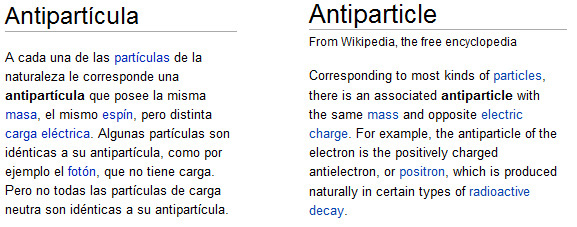
\includegraphics[width=\textwidth]{images/wiki.jpg}
\caption{An example of a Spanish/English document pair from Wikipedia.}
\label{fig:wiki}
\end{figure*}

Each document pair contains a sequence of source sentences (denoted by ${\bf
S}$) and target sentences (denoted by ${\bf T}$). Individual source and target
sentences are referred to by $S$ and $T$ respectively. Similarly, we refer to
the words within source and target sentences with the lowercase $s$ and $t$. We
borrow the notation of \citep{Och03} for describing alignments between sentences
as subsets of the Cartesian product of sentence positions. Sentence alignments
are referred to with the uppercase $A$, and word alignments with the lowercase
$a$.

The goal of sentence alignment is to identify which sentence pairs in the
bilingual document pairs are parallel. We view this as a retrieval task for
parallel sentence pairs, and so when annotated sentence alignments are present,
we can compute precision, recall, and F-measure.


\setcounter{chapter}{1}
\chapter{Related Work}
\label{chap:related_work}

Research in statistical machine translation (SMT) began as large parallel
corpora became available. These corpora include the Canadian Hansards
(French-English parliament proceedings) and the Hong Kong Laws Corpus, among many
others. While these corpora were parallel in the sense that they were created by
directly translating text in one language, they were not sentence aligned. Noise
in the form of missing data or sentences without a $1:1$ correspondence made
alignment a non-trivial problem. This lead to the development of several
approaches for aligning parallel corpora in the early 1990s. We will give an
overview of these approaches in Section \ref{sec:parallel_related}.

In addition to aligning parallel texts, there has also been a considerable
amount of work done on finding parallel sentence pairs in comparable corpora. A
comparable corpus is a multilingual collection of documents which may contain
parallel sentences, but is not completely parallel. This broad definition
includes both weakly aligned data such as timestamped multilingual news feeds,
and Wikipedia articles linked at the document level. Depending on the type of
comparable corpus, different methods may be more or less effective for finding
parallel sentences. We will split our review of comparable corpora mining
methods into two categories. In Section \ref{sec:noisy_related}, we will examine
methods used on closely aligned comparable corpora, and in Section
\ref{sec:nonnoisy_related} we will review work on extracting parallel sentences
from less related multilingual documents.

\section{Parallel Corpus Alignment}
\label{sec:parallel_related}

%\paragraph{Length based alignment}
Perhaps the most well known work on parallel corpus alignment is \citet{Gale91,Gale93}.
The authors described a sentence alignment method based on dynamic programming
which used only sentence length to determine whether or not two sentences were
parallel. This method is widely applicable since it assumes almost no linguistic
knowledge.\footnote{The only bit of information about the language pair required
is a ratio of sentence lengths in characters.} Despite this, it achieved very
high accuracy on a corpus of economic reports from the Union Bank of Switzerland
in English, French and German. \citet{Brown91} had a similar approach, using
only sentence lengths to align parallel corpora, but they measured length in
words rather than characters.

%\paragraph{Cognates}
Even when there is no bilingual lexicon available for a language pair, if the
source and target languages are similar enough it may be possible to use the
surface similarity of words to infer cognates. \citet{Simard93} made use of this
by replacing the length based alignment scoring of \citet{Gale93} with a cognate
based scoring method using a simple method for identifying cognates.
\citet{Church93} made use of cognates with a radically different approach:
creating a dotplot of character $n$-gram matches weighted by inverse frequency,
and then finding an alignment which best matches the dots. While this cognate
based approach was intended to work for similar languages, the authors noted
that even in language pairs like Japanese-English, matches can be found on
technical terms and markup.

%\paragraph{Inferring a bilingual dictionary}
The sentence alignment approach of \citet{Kay93} also used little linguistic
knowledge, though they build a bilingual dictionary from the parallel text to
facilitate alignment. Beginning with an initial set of sentence alignments, they
iteratively update the bilingual dictionary and the sentence alignments in a
manner similar to Viterbi EM, though no explicit probability model is given.
\citet{Chen93} had a similar approach, except he
incorporated the learning of both sentence and word alignments into a
probabilistic model. While this is similar to our work in that there is a
generative story of document pairs used to infer sentence alignments,
\citet{Chen93} used a joint probability distribution of source/target sentence
pairs which must be approximated for efficient inference, and several choices
are made in the inference strategy which assume a strongly monotonic sentence
alignment. Stochastic Viterbi EM is used to find the best sentence alignment.
% TODO: Make sure I'm being fair to Chen93, maybe reword

%\paragraph{Vector-based similarity}
As an alternative method for creating a bilingual dictionary, \citet{Fung94}
built a vector for each source/target word representing how it is distributed in
the parallel corpus. The intuition was that since the alignment between the
source and target data was strongly monotonic, so words that appear in the same
relative positions in the source/target corpora are likely to be translations of
one another.

%\paragraph{Bootstrapping}
\citet{Moore02} builds off of the length based alignment approach of
\citet{Gale93} by adding a bootstrapping step after the initial alignment.
First, a length based sentence alignment is done on the parallel corpus. Then,
the sentences found to be parallel are used to train a word alignment model
(IBM Model 1), and the sentence alignment dynamic program is repeated using
the word alignment scores in addition to length based scores. This bootstrapping
approach is popular in work on mining noisy parallel/comparable corpora (see
Section \ref{sec:comparable_related}).

\section{Comparable Corpus Mining}
\label{sec:comparable_related}

\subsection{Noisy Parallel Corpora}
\label{sec:noisy_related}
The first category of work on comparable corpora mining that we will review is
on noisy parallel data. While even corpora called ``parallel'' contain some
noise, we are refering to corpora which the methods in Section
\ref{sec:parallel_related} would fail on.

Similar to the dynamic programming approaches explored in Section
\ref{sec:parallel_related}, \citet{Zhao02} used a dynamic programming strategy
for aligning parallel sentences in a document pair. They create a probabilistic
model of a comparable document pair $P(S,T,A)$ and choose an alignment to
maximize the probability of the observed source and target documents. To
estimate the probability of two sentences being aligned, they used and IBM-style 
word alignment models (Model 3, specifically) which were estimated on existing
parallel data. \citet{Zhao02} also describes a bootstraping approach where high
confidence sentence alignments are added to the training data for the word
alignment model, and then sentence alignments are recomputed. Much of the work
on noisy parallel/comparable corpora mining used this technique 
\citep{Fung04a,Fung04b,Wu05,Munteanu05}.

\subsection{Comparable Corpora}
\label{sec:nonnoisy_related}
In comparable corpora such as bilingual news feeds or websites, the document
alignment is often not given.\footnote{A notable exception to this is Wikipedia}
First, we will review methods for finding comparable document pairs in a
comparable corpus, and then methods for identifying parallel sentence pairs
within these documents.

\subsubsection{Finding Comparable Document Pairs}
% Doc similarity (Munteanu, Fung)
The Gigaword corpus contains news feeds in multiple languages, and is annotated
with the date of publication. Since these news articles are potentially on the
same topic, there are potentially parallel sentence pairs in these articles.
\citet{Munteanu04,Munteanu05, Fung04a, Fung04b} make use of this information to
find comparable document pairs. The basic strategy is to first consider all
bilingual article pairs published within a time window to be potentially
comparable. Then, documents in one language are projected through a bilingual
dictionary, and bag-of-words based document similarity measures are used to
prune this large set of document pairs. This requires either existing parallel
data or at least a bilingual dictionary. Document pairs that pass through these
filter are then mined for parallel sentences.

% STRAND
Multilingual websites are another potential source for comparable or parallel
document pairs. STRAND \citep{Resnik03} used some heuristics for identifying
links between versions of the same website in different languages. This provides
a candidate set of document pairs, which are further filtered by looking at
their HTML structure. Each website is converted into a list of start tags, end
tags, and ``chunks'' (text within a tag), and these lists are aligned using
standard dynamic programming techniques. This alignment is not only used to
determine whether a pair of websites is comparable, but it also gives an
alignment of text chunks which greatly narrows down the space of possible
sentence alignments

A drastically different approach for finding parallel web pages is given by 
\citet{Uszkoreit10}. Using a existing language identification and translation
systems, they identify the language of all webpages and translate the
non-English ones into English. Since all documents are now in the same language,
the problem of identifying comparable webpages is treated as near-duplicate
detection. An index is built mapping $n$-grams to documents, and this index is
used to find a bag-of-$n$-grams score for potentially comparable documents. The
computation is kept feasible by only creating index entries for rare $n$-grams.

\subsubsection{Finding Parallel Sentences}
Once comparable document pairs have been identified, most comparable corpora
extraction methods will independently judge each sentence pair as parallel or
non-parallel. Since there is often a very large amount of document pairs and
thus potential sentence pairs, filters are used to prune out sentence pairs that
are highly unlikely to be parallel. For example, \citet{Munteanu05} used a
sentence length filter to remove sentence pairs where one sentence was more than
twice as long as the other. In addition, they used a word overlap filter based
on the bilingual dictionary used to find candidate document pairs.

Given a filtered set of sentence pairs, more expensive methods of scoring
sentence pairs can be used. \citet{Munteanu05} use a MaxEnt binary MaxEnt
classifier to ultimately determine whether or not a sentence pair is parallel.
The classifier is trained on parallel data and makes used of features which are
mostly based on word alignments. Others
\cite{Fung04a,Fung04b,Tillmann09a,Tillmann09b} use a single score for sentence
pairs based on either a word alignment model or bag-of-words similarity after
projection through a bilingual lexicon, and tune a threshold on held out data.

% Sub-sentence alignment?


\setcounter{chapter}{2}
\chapter{Mining Parallel Data from the Web}
\label{chap:web}



\setcounter{chapter}{3}
\chapter{Discriminative Sentence Alignment}
\label{chap:supervised}

In this chapter we will describe a discriminative model for performing sentence
alignment on comparable document pairs. We use Wikipedia as our source for
comparable documents.

\section{Wikipedia as a Comparable Corpus}
\label{sec:wiki}
Wikipedia \citep{wikipedia} is an online collaborative encyclopedia available in
a wide variety of languages.  While the English Wikipedia is the largest, with
over 3 million articles, there are 24 language editions with at least 100,000
articles.

Articles on the same topic in different languages are also connected via
``interwiki'' links, which are annotated by users.  This is an extremely
valuable resource when extracting parallel sentences, as the document alignment
is already provided.  
Table \ref{table:interwiki} shows how
many of these ``interwiki'' links are present between the English Wikipedia and the
16 largest non-English Wikipedias.

\begin{table*}
\begin{center}
\begin{tabular}{|c|c|c|c|c|c|c|c|}
\hline
French & German & Polish & Italian & Dutch & Portuguese & Spanish & Japanese \\
496K & 488K & 384K & 380K & 357K & 323K & 311K & 252K\\
\hline
Russian & Swedish & Finnish & Chinese & Norwegian & Volap\"{u}k & Catalan & Czech \\
232K & 197K & 146K & 142K & 141K & 106K & 103K & 87K\\
\hline
\end{tabular}
\end{center}
\caption{Number of aligned bilingual articles in Wikipedia by language (paired with English).}
\label{table:interwiki}
\end{table*}

Wikipedia's markup contains other useful indicators for parallel sentence
extraction.  The many hyperlinks found in articles have previously been used as
a valuable source of information.  \citep{Adafre06} use matching
hyperlinks to identify similar sentences.  Two links match if the articles they
refer to are connected by an ``interwiki'' link.
Also, images in Wikipedia are often stored in a central source across
different languages; this allows identification of captions which may be
parallel.  Finally, there are other minor forms
of markup which may be useful for finding similar content across languages, such
as lists and section headings.  In Section \ref{sec:features}, we will explain
how features are derived from this markup.

\section{Models for Parallel Sentence Extraction}
\label{sec:models} In this section, we will focus on methods for
extracting parallel sentences from aligned, comparable documents.
The related problem of automatic document alignment in news and
web corpora has been explored by a number of researchers,
including
\citet{Resnik03}, \citet{Munteanu05},
\citet{Tillmann09a}, and \citet{Tillmann09b}.
Since our corpus already contains document alignments, we sidestep
this problem, and will not discuss further details of this issue.
That said, we believe that our methods will be effective in
corpora without document alignments when combined with one of the
aforementioned algorithms.


\subsection{Binary Classifiers and Rankers}
Much of the previous work involves building a binary classifier for sentence
pairs to determine whether or not they are parallel
\citep{Munteanu05,Tillmann09a}.
The training data usually comes from a standard parallel corpus.  There is a
substantial class imbalance ($O(n)$ positive examples, and $O(n^2)$
negative examples), and various heuristics are used to mitigate this problem.
\citet{Munteanu05} filter out negative
examples with high length difference or low word overlap (based on a bilingual
dictionary).

We propose an alternative approach: we learn a ranking model, which, for each sentence in the {\em
source} document, selects either a sentence in the {\em target} document that it is
parallel to, or ``null''.
This formulation of the problem avoids the class imbalance issue of the binary classifier.

In both the binary classifier approach and the ranking approach, we use a Maximum Entropy
classifier, following \citet{Munteanu05}.

\subsection{Sequence Models}
In Wikipedia article pairs, it is common for parallel sentences to
occur in clusters.  A global sentence alignment model is
able to capture this phenomenon. For both parallel and comparable
corpora, global sentence alignments have been used, though the
alignments were monotonic
\citep{Gale93,Moore02,Zhao02}.
Our model is a first order linear chain Conditional Random Field
(CRF) \citep{Lafferty01}. The set of source and
target sentences are observed. For each {\em source} sentence, we
have a hidden variable indicating the corresponding {\em target}
sentence to which it is aligned (or null). The model is similar to the
discriminative CRF-based word alignment model of
\citep{Blunsom06}.

\subsection{Features}
\label{sec:features}
Our features can be grouped into four categories.

\subsubsection{Features derived from word alignments}
%kristina-edit-1

We use a feature set inspired by \citep{Munteanu05}, who defined
features primarily based on IBM Model 1 alignments
\citep{Brown93}.  We also use HMM word alignments
\citep{Vogel96} in both directions ({\em source} to {\em target} and
{\em target} to {\em source}), and extract the following features based on these
four alignments:\footnote{These are all derived from the one best alignment, and
normalized by sentence length.}

\begin{enumerate}
\item Log probability of the alignment
\item Number of aligned/unaligned words
\item Longest aligned/unaligned sequence of words
\item Number of words with fertility 1, 2, and 3+
\end{enumerate}

We also define two more features which are independent of word alignment
models.  One is a sentence length feature taken from \citep{Moore02}, which
models the length ratio between the {\em source} and {\em target} sentences with
a Poisson distribution.  The other feature is the difference in relative
document position of the two sentences, capturing the idea that the aligned
articles have a similar topic progression.

The above features are all defined on sentence pairs, and are included in the
binary classifier and ranking model.
\subsubsection{Distortion features} In the sequence model, we use additional distortion
features, which only look at the difference between the position
of the previous and current aligned sentences.  One set of
features bins these distances; another looks at the
absolute difference between the expected position (one after the
previous aligned sentence) and the actual position.

\subsubsection{Features derived from Wikipedia markup}

Three features are derived from Wikipedia's
markup. The first is the number of matching links in the sentence
pair. The links are weighted by their inverse frequency in the
document, so a link that appears often does not contribute much to
this feature's value.  The image feature fires whenever two
sentences are captions of the same image, and the list feature
fires when two sentences are both items in a list.  These last two
indicator features fire with a negative value when the feature
matches on one sentence and not the other.

None of the above features fire on a null alignment, in either the
ranker or CRF.  There is also a bias feature for these two models, which
fires on all non-null alignments.

\subsubsection{Word-level induced lexicon features}
In order to address sparsity issues in our seed parallel corpora, we introduce a
bilingual lexicon model which learns word translation probabilities from the
linked Wikipedia articles. The details of this model and the features derived
from it can be found in \citep{Smith10}.

\section{Experiments}
\label{sec:exp}

\subsection{Data}
We annotated twenty Wikipedia article pairs for three language pairs: Spanish-English,
Bulgarian-English, and German-English.
Each sentence in the {\em source} language was annotated with
possible parallel sentences in the {\em target} language (the target language was
English in all experiments).  The pairs were annotated with a quality level:
{\bf 1} if the sentences contained some parallel fragments, {\bf 2} if the sentences
were mostly parallel with some missing words, and {\bf 3} if the sentences appeared to be direct
translations.  In all experiments, sentence pairs with quality {\bf 2} or {\bf 3} were
taken as positive examples. 

\begin{table*}[ht]
\begin{center}
\begin{tabular}{|c||c|c|c||c|c|c||c|c|c|}
\hline
Language Pair     & \multicolumn{3}{|c||}{Binary Classifier} & \multicolumn{3}{|c||}{Ranker} & \multicolumn{3}{|c|}{CRF} \\
\hline
                  & Avg Prec & R@90 & R@80
                  & Avg Prec & R@90 & R@80
                  & Avg Prec & R@90 & R@80 \\
\hline
\footnotesize{English-Bulgarian} & 75.7  & 33.9  & 56.2    & 76.3  & 38.8  & 57.0    & {\bf 80.6}  & {\bf 52.9}  & {\bf 59.5} \\
\footnotesize{English-Spanish}   & 90.4  & 81.3  & 87.6    & 93.4  & 81.0  & 84.5    & {\bf 94.7}  & {\bf 87.6}  & {\bf 90.2} \\
\footnotesize{English-German}    & 61.8  &  9.4  & 27.5    & 66.4  & 25.7  & 42.4    & {\bf 78.9}  & {\bf 52.2}  & {\bf 54.7} \\
\hline
\end{tabular}
\end{center}
\caption{Average precision, recall at 90\% precision, and recall at 80\%
precision for each model in all three language pairs.  In these experiments, the
Wikipedia features and lexicon features are omitted.}
\label{table:modelcompare}
\end{table*}

\begin{table*}[ht]
\begin{center}
\begin{tabular}{|c||c|c|c||c|c|c|}
\hline
Setting           & \multicolumn{3}{|c||}{Ranker} & \multicolumn{3}{|c|}{CRF} \\
\hline
                  & Avg Prec & R@90 & R@80
                  & Avg Prec & R@90 & R@80\\
\hline
English-Bulgarian & & & & & & \\
\hline
One Direction          & 76.3  & 38.8  & 57.0    & 80.6  & 52.9  & 59.5 \\
Intersected            & 78.2  & 47.9  & 60.3    & 79.9  & 38.8  & 57.0 \\
Intersected +Wiki      & 80.8  & 39.7  & 68.6    & 82.1  & 53.7  & 62.8 \\
Intersected +Wiki +Lex & 89.3  & 64.4  & 79.3    & {\bf 90.9}  & {\bf 72.0}  & {\bf 81.8} \\
\hline
English-Spanish & & & & & & \\
\hline
One Direction          & 93.4  & 81.0  & 84.5    & 94.7  & 87.6  & 90.2 \\
Intersected            & 94.3  & 82.4  & 89.0    & 95.4  & 88.5  & 91.8 \\
Intersected +Wiki      & 94.5  & 82.4  & 89.0    & 95.6  & 89.2  & 92.7 \\
Intersected +Wiki +Lex & 95.8  & 87.4  & 91.1    & {\bf 96.4}  & {\bf 90.4}  & {\bf 93.7} \\
\hline
English-German & & & & & & \\
\hline
One Direction          & 66.4  & 25.7  & 42.4    & 78.9  & 52.2  & 54.7 \\
Intersected            & 71.9  & 36.2  & 43.8    & 80.9  & 54.0  & 67.0 \\
Intersected +Wiki      & 74.0  & 38.8  & 45.3    & 82.4  & 56.9  & {\bf 71.0} \\
Intersected +Wiki +Lex & 78.7  & 46.4  & 59.1    & {\bf 83.9}  & {\bf 58.7}  & 68.8 \\
\hline
\end{tabular}
\end{center}
\caption{Average precision, recall at 90\% precision, and recall at 80\%
precision for the Ranker and CRF in all three language pairs.  ``+Wiki''
indicates that Wikipedia features were used, and ``+Lex'' means the lexicon
features were used.}
\label{table:featurecompare}
\end{table*}



For our seed parallel data, we used the Europarl corpus
\citep{Koehn05} for Spanish and German and the
JRC-Aquis corpus for Bulgarian, plus the article titles for
parallel Wikipedia documents, and translations available from
Wiktionary entries.\footnote{Wiktionary is an online collaborative
dictionary, similar to Wikipedia.} %kristina-edit

\subsection{Intrinsic Evaluation}
Using 5-fold cross-validation on the 20 document pairs for each
language condition, we compared the binary classifier, ranker, and
CRF models for parallel sentence extraction. To tune for 
precision/recall, we used minimum Bayes risk decoding.  We define
the loss $L(\tau,\mu)$ of picking target sentence $\tau$ when the
correct target sentence is $\mu$ as $0$ if $\tau=\mu$, $\lambda$ if
$\tau = \textsc{null}$ and $\mu\ne\textsc{null}$, and $1$ otherwise.
By modifying the null loss $\lambda$, the precision/recall
trade-off can be adjusted.  For the CRF model, we used posterior
decoding to make the minimum risk decision rule tractable. As a
summary measure of the performance of the models at different
levels of recall we use average precision as defined in
\citep{Ido06}. We also report recall at precision of 90 and
80 percent. %kristina-edit 
 Table \ref{table:modelcompare} compares the
different models in all three language pairs.

In our next set of experiments, we looked at the effects of the Wikipedia
specific features.  Since the ranker and CRF are asymmetric models,
we also experimented with running the models in both directions and combining
their outputs by intersection.  These results are shown in Table \ref{table:featurecompare}.

Identifying the agreement between two asymmetric models is a commonly
exploited trick elsewhere in machine translation. It is mostly effective
here as well, improving all cases except for the Bulgarian-English CRF where
the regression is slight. More successful are the Wikipedia features, which
provide an auxiliary signal of potential parallelism.

The gains from adding the lexicon-based features can be dramatic
as in the case of Bulgarian (the CRF model average precision
increased by nearly 9 points). The lower gains on Spanish and
German may be due in part to the lack of language-specific
training data. These results are very promising and
motivate further exploration. We also note that this
is perhaps the first successful practical application of an
automatically induced word translation lexicon.

\subsection{SMT Evaluation}

We also present results in the context of a full machine translation system
to evaluate the potential utility of this data.  A standard
phrasal SMT system \citep{Koehn03} serves as our testbed, using
a conventional set of models: phrasal models of source given target and
target given source; lexical weighting models in both directions, language
model, word count, phrase count, distortion penalty, and a lexicalized
reordering model.  Given that the extracted Wikipedia data takes the
standard form of parallel sentences, it would be easy to exploit this same
data in a number of systems.

\begin{table*}[ht]
\begin{center}
\begin{tabular}{|rr||r|r||r|r||r|r|}
\hline
      &                & German        & English       & Spanish       & English      & Bulgarian    & English   \\
\hline
      & sentences     & 924,416       & 924,416       & 957,884       & 957,884      & 413,514      & 413,514   \\
\textbf{Medium} \
      & types     & 351,411       & 320,597       & 272,139       & 247,465      & 115,756      & 69,002    \\
      & tokens    & 11,556,988    & 11,751,138    & 18,229,085    & 17,184,070   & 10,207,565   & 10,422,415\\
\hline
      & sentences      & 6,693,568     & 6,693,568     & 7,727,256     & 7,727,256    & 1,459,900    & 1,459,900 \\
\textbf{Large} \
      &      types     & 1,050,832     & 875,041       & 1,024,793     & 952,161      & 239,076      & 137,227   \\
      &      tokens    & 100,456,622   & 96,035,475    & 155,626,085   & 137,559,844  & 29,741,936   & 29,889,020\\
\hline
      & sentences      & 1,694,595     & 1,694,595     & 1,914,978     & 1,914,978    & 146,465      & 146,465   \\
\textbf{Wiki}  \
      &      types     & 578,371       & 525,617       & 569,518       & 498,765      & 107,690      & 74,389    \\
      &      tokens    & 21,991,377    & 23,290,765    & 29,859,332    & 28,270,223   & 1,455,458    & 1,516,231 \\
\hline
\end{tabular}
\end{center}
\caption{Statistics of the training data size in all three language pairs.}
\label{table:mtTrainStats}
\end{table*}

\begin{table*}[ht]
\begin{center}
\begin{tabular}{|rr||r|r||r|r||r|r|}
\hline
      &                & German        & English       & Spanish       & English      & Bulgarian     & English   \\
\hline
\textbf{Dev A} \
      & sentences      & 2,000         & 2,000         & 2,000         & 2,000        & 2,000         & 2,000     \\
      & tokens    & 16,367        & 16,903        & 24,571        & 21,493       & 39,796        & 40,503    \\
\hline
\textbf{Test A}\
      & sentences      & 5,000         & 5,000         & 5,000         & 5,000        & 2,473         & 2,473     \\
      & tokens    & 42,766        & 43,929        & 68,036        & 60,380       & 52,370        & 52,343    \\
\hline
\textbf{Wikitest}\
      & sentences    & 500           & 500           & 500           & 500          & 516           & 516       \\
      & tokens    & 8,235         & 9,176         & 10,446        & 9,701        & 7,300         & 7,701     \\
\hline
\end{tabular}
\end{center}
\caption{Statistics of the test data sets.}
\label{table:mtTestStats}
\end{table*}

For each language pair we explored two training conditions.  The
``Medium'' data
condition used easily downloadable corpora: Europarl for German-English and
Spanish-English, and JRC/Acquis for Bulgarian-English.  Additionally we
included titles of all linked Wikipedia articles as parallel sentences in
the medium data condition.  The ``Large'' data condition includes all the
medium
data, and also includes using a broad range of available sources such as
data scraped from the web~\citep{Resnik03}, data from the United
Nations, phrase books, software documentation, and more.

In each condition, we explored the impact of including additional
parallel sentences automatically extracted from Wikipedia in the
system training data. For German-English and Spanish-English, we
extracted data with the null loss adjusted to
achieve an estimated precision of 95 percent, and for
English-Bulgarian a precision of 90 percent. %kristina-edit-1
Table~\ref{table:mtTrainStats} summarizes the characteristics of
these data sets.  We were pleasantly surprised at the amount of
parallel sentences extracted from such a varied comparable corpus.
Apparently the average Wikipedia article contains at least a
handful of parallel sentences, suggesting this is a very fertile
ground for training MT systems.

The extracted Wikipedia data is likely to make the greatest impact on broad
domain test sets -- indeed, initial experimentation showed little BLEU gain
on in-domain test sets such as Europarl, where out-of-domain training data
is unlikely to provide appropriate phrasal translations.  Therefore, we
experimented with two broad domain test sets.

First, Bing Translator provided a sample of translation
requests along with translations in German-English and
Spanish-English -- this constituted our standard development and
test set for those language pairs.  Unfortunately no such tagged
set was available in Bulgarian-English, so we held out a portion
of the large system's training data to use for development and
test. In each language pair, the test set was split into a
development portion (``Dev A'') used for minimum error rate
training~\citep{OchMert03} and a test set (``Test A'') used
for final evaluation.

\begin{table*}[ht!]
\begin{center}
\begin{tabular}{|lr||l||l|l|}
\hline
Language pair     & Training data     & Dev A             & Test A            & Wikitest     \\
\hline
Spanish-English   & Medium            & 32.6              & 30.5              & 33.0         \\
                  & Medium+Wiki       & 36.7 (+4.1)       & 33.8 (+3.3)       & 39.1 (+6.1)  \\
                  & Large             & 39.2              & \textbf{37.4}     & 38.9         \\
                  & Large+Wiki        &\textbf{39.5} (+0.3)&37.3 (-0.1)       & \textbf{41.1} (+2.2)  \\
\hline
German-English    & Medium            & 28.7              & 26.6              & 13.0         \\
                  & Medium+Wiki       & 31.5 (+2.8)       & 29.6 (+3.0)       & 18.2 (+5.2)  \\
                  & Large             & \textbf{35.0}     & 33.7              & 17.1         \\
                  & Large+Wiki        & 34.8 (-0.2)       &\textbf{33.9} (+0.2)&\textbf{20.2} (+3.1)  \\
\hline
Bulgarian-English & Medium            & 36.9              & 26.0              & 27.8         \\
                  & Medium+Wiki       & 37.9 (+1.0)       & 27.6 (+1.6)       & 37.9 (+10.1) \\
                  & Large             &\textbf{51.7}      &\textbf{49.6}      & 36.0         \\
                  & Large+Wiki        &\textbf{51.7}(+0.0)& 49.4 (-0.2)       &\textbf{39.5}(+3.5)  \\
\hline
\end{tabular}
\end{center}
\caption{BLEU scores of MT systems under various training and test
conditions.  The final BLEU score from minimum error rate training is in the
first column; two additional columns are BLEU scores on held-out test sets.
For training data conditions including the extracted Wikipedia sentences,
the parenthesized values indicate the absolute BLEU difference against the
corresponding system without Wikipedia extracts.}
\label{table:mtTestResults}
\end{table*}

Second, we created new test sets in each of the three language
pairs by sampling parallel sentences from held out Wikipedia
articles.  To ensure that this test data was clean, we manually
filtered the sentence pairs that were not truly parallel and
edited them as necessary to improve adequacy.  We called
this ``Wikitest''. Characteristics of
these test sets are summarized in Table~\ref{table:mtTestStats}.

We evaluated the resulting systems using
BLEU-4~\citep{Papineni02}; the results are presented in
Table~\ref{table:mtTestResults}.  First we note that the extracted
Wikipedia data are very helpful in medium data conditions,
significantly improving translation performance in all conditions.
Furthermore we found that the extracted Wikipedia sentences
substantially improved translation quality on held-out Wikipedia
articles. In every case, training on medium data plus Wikipedia
extracts led to equal or better translation quality than the large
system alone. Furthermore, adding the Wikipedia data to the large
data condition still made substantial improvements.


\setcounter{chapter}{4}
\chapter{Comparable Data on Twitter}
\label{chap:twitter}

Methods for mining comparable corpora often leverage any available annotation
which may assist in finding parallel data. 
Many Web mining methods find parallel documents through their hyperlinks or
URLs \citep{Nie99,Chen00,Resnik99,Resnik03,Smith13}. \citet{Munteanu05} make use of the
publication date of news articles to narrow down the set of document pairs to
consider. Wikipedia contains ``interwiki links'' which directly identify
articles on the same topic in different languages, and within the articles,
other forms of markup such as links or images can help identify which
sentences are parallel \citep{Smith10}.
%While some methods avoid use of any
%annotation and work only with the text of the documents, they tend to be
%computationaly prohibitive \citep{Uszkoreit10,Ture12}.

\section{Related Work}
% Doc similarity (Munteanu, Fung)
The Gigaword corpus contains news feeds in multiple languages, and is annotated
with the date of publication. Since these news articles are potentially on the
same topic, there are potentially parallel sentence pairs in these articles.
\citet{Munteanu04,Munteanu05, Fung04a, Fung04b} make use of this information to
find comparable document pairs. The basic strategy is to first consider all
bilingual article pairs published within a time window to be potentially
comparable. Then, documents in one language are projected through a bilingual
dictionary, and bag-of-words based document similarity measures are used to
prune this large set of document pairs. This requires either existing parallel
data or at least a bilingual dictionary. Document pairs that pass through these
filter are then mined for parallel sentences.

% STRAND
Multilingual websites are another potential source for comparable or parallel
document pairs. STRAND \citep{Resnik03} used some heuristics for identifying
links between versions of the same website in different languages. This provides
a candidate set of document pairs, which are further filtered by looking at
their HTML structure. Each website is converted into a list of start tags, end
tags, and ``chunks'' (text within a tag), and these lists are aligned using
standard dynamic programming techniques. This alignment is not only used to
determine whether a pair of websites is comparable, but it also gives an
alignment of text chunks which greatly narrows down the space of possible
sentence alignments

A drastically different approach for finding parallel web pages is given by 
\citet{Uszkoreit10}. Using a existing language identification and translation
systems, they identify the language of all webpages and translate the
non-English ones into English. Since all documents are now in the same language,
the problem of identifying comparable webpages is treated as near-duplicate
detection. An index is built mapping $n$-grams to documents, and this index is
used to find a bag-of-$n$-grams score for potentially comparable documents. The
computation is kept feasible by only creating index entries for rare $n$-grams.

\citet{Ture12} used cross-lingual information retrieval techniques to find
comparable document pairs in Wikipedia. While Wikipedia already provides
annotated comparable document pairs through interwiki links, the authors
consider all possible German-English article pairs as potentially containing
comparable data.

\subsection{Twitter}
Twitter is an interesting case, as its ``documents'' (tweets) are only 140 characters
long, and usually a single sentence at most. Tweets also contain many
potentially useful annotations: the author, the time it was posted, the names of
other users mentioned, and hashtags, which are informal topic annotations
({\tt \#worldcup}, for example). None of these are direct indicators that tweets
are parallel or even topic-aligned, but they still are useful in narrowing
the search space. 

% Prev. Twitter work (double check)
Previous work on mining parallel data from Twitter has used a
manually created list of terms associated with a topic that has multilingual
coverage \citep{Jehl12}, or searched for parallel
data within individual tweets \citep{Ling13}. We are interested in a general
methods for finding parallel tweets which do not require any initial knowledge
of topics.

In order to make the best use of the annotations available on Twitter, we
characterize the different sources of parallel data. Bilingual users may post
the same content in two languages, or directly translate another tweet. In
addition to these intentional translations, we also find coincidental
translations, where users independently tweet the same content about some
current event. These different types of parallel data are found by leveraging
different signals from Twitter. For each of these signals, we would like to
answer a few questions: Which languages are represented? A monolingual author or
hashtag cannot contain any parallel data. Also, how likely are we to
find parallel data? The hashtag {\tt \#no} will likely contain both Spanish and
English data, but not much of it will be parallel.

We use these signals to align potentially parallel tweets, and apply a
supervised classifier \citep{Munteanu05} to determine which pairs are actually parallel.
To test the quality of this data, we include SMT experiments which compare a
system trained with baseline data against one with our mined data added. We
assemble a test set of parallel tweets from GlobalVoices\footnote{{\tt globalvoicesonline.org}}
and show an improvement of X BLEU.

\section{Parallel and Comparable Tweets}
The term ``comparable corpus'' describes a wide array of multilingual corpora with varying
degrees of correspondence. \citet{Fung04a} give a more fine-grained
categorization based on the degree of topic-alignment and whether or not the
corpus was created by direct translation. When searching for parallel data on
Twitter, we will make the distinction between tweet pairs that are intentionally
translated, and pairs that are coincidentally translations. For example, many
Twitter users tweet the same information in multiple languages, on one or more
feeds, which gives us intentionally translated text. Users may also
independently tweet about some current event, and coincidentally convey the same
information. Figure \ref{tab:ex_tweets} shows examples of each.

\begin{table*}
\begin{tabular}{|c|c|}
\hline
English & can u listen to my song please? \\
\hline
Spanish & puede escuchar mi canci\'{o}n? \\
\hline
\hline
English & RT @celtics : Kobe Bryant surpassed Michael Jordan as the all-time NBA
\#AllStar scorer tonight.\\
\hline
Spanish & \#KobeBryant m\'{a}s puntos en \#AllStar games de todos los tiempos. :')\\
\hline
\hline
English & @NiallOfficial I love you, and do not lose faith that someday answer
me x9.\\
\hline
Spanish & @NiallOfficial te amo, y no pierdo la fe de que algu ́n día me
respondas.\\
\hline
\end{tabular}
\caption{Examples of intentional and coincidental translations on Twitter. The
first pair of tweets came from the same author, the second contained the
same hashtag ({\tt \#AllStar}), and the third contained the same mention ({\tt
@NiallOfficial}).}
\label{tab:ex_tweets}
\end{table*}

Naturally, we would expect different annotations on Twitter to be useful when
searching for intentional or coincidental translations. Looking at the author of
the tweet is important when searching for intentional translations. Other forms
of annotation, such as mentions, hashtags, and URLs are useful for aligning tweets by
topic. One important signal for finding any type of translation is the timestamp - we
expect translations to be published within a short timespan after the original
tweet.

Since we can't afford to search over all possible pairs of tweets, we use these
signals to narrow down the search space.
Similar to \citet{Munteanu05}, we use a sliding window when considering
candidate pairs of parallel tweets. In addition to this time-based matching, we
also require tweets to match in either their author, mention, hashtag, or URL to be
considered parallel.
We apply language identification \citep{Bergsma12} on matching sets of tweets to
further filter potential pairs to those in the correct source/target languages.

Once we have a filtered set of candidate pairs, we use the supervised classifier
of \citet{Smith10}, trained on their annotated Wikipedia data, to determine which
pairs are parallel.

\section{Notes}

\subsection{Matching Dimensions}
We align tweets by five dimensions: author, hashtag, mention, URL, and time.
We never use time alone to find parallel tweets - we use it to
further filter tweets matched by another attribute.

When matching tweets on the author attribute, we are attempting to find examples
of authors translating their own tweets into one or more other languages. We
expect that the translations will follow within a few minutes of the original tweet,
so a large time window is not required. We can also narrow down the search for
parallel tweets by only considering authors who regularly tweet in multiple
languages.

Hashtags are user-created topic markers. They have become used for things not
traditionally considered topics, such as {\tt \#ff} (follow Friday), or {\tt
\#sorrynotsorry}. We expect to find parallel tweets only from hashtags which
are related to current events, such as awards ceremonies ({\tt \#goldenglobes}),
sporting events ({\tt \#allstars}), and elections ({\tt \#Obama2012}).
We expect hashtags whose usage spikes at the same time in multiple languages to
be good potential sources of parallel data.

Tweets containing the same mentions ({\tt @user}) are not expected to be
parallel unless the user being mentioned is some public figure which many users
are likely to talk about. Actors, atheletes, and politicians are good potential
candidates for having a large multi-lingual following. We look for users who
have a high follower count and frequent mentions in our sample of tweets.

URLs are one source of matching tweets that is potentially independent of time:
two users may see an article at different times and tweet summaries in different
languages. Tweets containing the same URL are relatively rare, so even though
this is a strong signal that the tweets convey the same information, we don't
find large amounts of parallel data from this attribute.

There are some other attributes included in tweets which we decided not to use
for matching. When a tweet is created as a reply, it contains a reference to the
original. It also automatically includes a mention of the user being replied to,
so reply information was left out as redundant. Other metadata associated with a
tweet, such as the number of favorites, are not useful in matching potentially
parallel tweets.
% TODO: Check the auto-mention in replies


\section{Results}
We use a collection of tweets from Twitter's sample stream from 2012 (X
tweets total) as our input data. Our extraction algorithm is as follows:

\begin{enumerate}
\item Filter tweets for length and content---they must include at least five
tokens containing alphabetical characters, and excluding Twitter markup \adlul{such as}\adlmp{Be concrete. Is this everything you ignore?}
mentions and hashtags.
\item Perform language identification on the remaining tweets, and discard those
\adlul{not in the source or target language}.\adlmp{Is there some threshold?}
\item Index the remaining tweets by their attributes and a timestamp. The time
stamp is created by taking the time the tweet was posted, converting it to an
integer number of minutes, and dividing by the length of the time window (30
minutes in our experiments). Each tweet indexed by its current timestamp and the
immediately preceding one to ensure that tweets near time window boundaries are
correctly matched.\NoteJS{This needs a diagram to be explained clearly}
\item Apply a supervised parallel sentence classifier \citep{Smith10} to source and target tweets
that match on any attribute.\adlmp{after wikipedia chap.}
\item Remove \adlul{duplicated sentences pairs}\adlmp{Are there many?} from the resulting parallel data.
\end{enumerate}

Table \ref{tab:data_results} shows how much parallel data we find
for Spanish-English.

\begin{table*}[ht]
\begin{center}
\begin{tabular}{|c||c|c|}
\hline
Language & Segments & Tokens \\
\hline
\hline
English & 64,985 & 1,210,051 \\
\hline
Spanish & 64,985 & 1,158,787 \\
\hline
\end{tabular}
\end{center}
\caption{The amount of English-Spanish parallel data mined from our sample of
tweets from 2012. While it is possible that a single tweet may contain more than
one sentence, we are treating each tweet as its own segment.}
\label{tab:tweet_data_results}
\end{table*}

\section{Conclusions}


\setcounter{chapter}{5}
\chapter{Unsupervised Parallel Sentence Extraction from Comparable Corpora}
\label{chap:unsupervised}

\section{Unsupervised Sentence Alignment}
\label{sec:alignment}
In most previous work on finding parallel sentences in comparable corpora, some
initial parallel data (parallel sentences or bilingual dictionary entries) is
used as a starting point. This data is used to extract parallel sentences, with
the hope that the bilingual word correspondences from the initial data are enough to
determine whether or not two sentences are parallel. The obvious drawback is
the reliance on the initial data, which may be small. Ideally, one would learn
additional word correspondences from parallel sentences that were extracted, and
this information could be used to find more parallel sentences. In fact, this
bootstrapping method has been used in previous work \citep{Fung04a,Fung04b,Wu05}.

We will explore a novel way of using semi-supervised learning to find
parallel sentences: by including sentence and word alignment in a single model.
Much like the IBM word alignment models \citep{Brown93} which can be trained on
sentence pairs without word alignment data, our model can be trained on document
pairs without sentence or word alignment data, and can similarly be trained using
the expectation-maximization (EM) algorithm \citep{Dempster77}.

\subsection{Model}

First we must define a generative model of a bilingual (possibly) parallel
document pair. We will use a joint model of the source and target documents
based on stochastic edit distance \citep{Ristad98}. Document pairs are
generated by a memoryless transducer which generates substitution pairs $(S,T)$,
insertion pairs $(\epsilon, T)$, deletion pairs $(S,\epsilon)$, and the
termination pair $(\epsilon, \epsilon)$, borrowing the convention used by
\citep{Oncina06} for simplicity. Substitution pairs correspond to parallel
source and target sentences, while the insertion and deletion pairs are
monolingually generated. For this model to be properly defined, the probability
of generating all pairs must sum to one:

\begin{equation}
\sum_{x \in S\cup \{\epsilon\}, y \in T\cup \{\epsilon\}} p(x,y) = 1
\end{equation}

Since the insertion and deletion operations are monolingual generation of
sentences, we use a standard $n$-gram language model for their probabilities.
For the probability of a substitution pair, we decompose $p(S,T)$ into
$p(T|S)p(S)$. $p(T|S)$ is defined by an IBM word alignment model \citep{Brown93}
(Model 1 in this preliminary work), and $p(S)$ is given by the same language
model used to generate deletion pairs ($(S,\epsilon)$). Since $p(S,T)$,
$p(S,\epsilon)$ and $p(\epsilon,T)$ all individually sum to one, they must be
weighted to ensure that $p({\bf S},{\bf T})$ is properly
normalized.\footnote{Since our document pairs are always observed, we can safely
ignore the stopping cost $p(\epsilon, \epsilon)$ by assuming it to be some small
constant.} In this work, we will use a single parameter to weight these pairs:

\begin{align*}
p(S,T) &=& \lambda p_{Model1}(T|S) p_{LM}(S)\\
p(S,\epsilon) &=& \frac{1-\lambda}{2} p_{LM}(S)\\
p(\epsilon,T) &=& \frac{1-\lambda}{2} p_{LM}(T)
\end{align*}

$p_{Model1}$ and $p_{LM}$ refer to the IBM Model 1 and a unigram language model,
respectively. The parameter $\lambda$ roughly controls how eager the model
is to label sentence pairs as parallel. This can be set based on some prior
knowledge about the corpus.
\remove{
We will explore additional methods for setting
$\lambda$ in Section \ref{sec:extensions}.
}
$p_{Model1}$ is given by the
following equation from \citep{Brown93}:

\begin{equation}
p(T|S) = p\left(|T|\big||S|\right) \frac{1}{|S|^{|T|}}
\prod_{j=1}^{|T|} \sum_{i=1}^{|S|} p(t_j|s_i)
\end{equation}

For simplicity, we assume the source sentence $S$ contains the null word. The
term $\frac{1}{|S|^{|T|}}$ is the uniform alignment probability. The
length distribution, $p\left(|T|\big||S|\right)$, was originally described as a uniform distribution
over a large finite set of lengths. Since Model 1 is usually applied to parallel
corpora with observed sentence alignments, and the goal of using Model 1 is to
find word translation probabilities ($p(t|s)$), it is unnecessary to find an
accurate model of sentence length. However, when the sentence alignments are
being learned, it is important to have an accurate model of the length of the
target sentence given the source sentence. In this work, we use a Poisson
distribution to model the target sentence length, following \citet{Moore02}.

The probability for generating sentences monolingually, $p_{LM}(S)$, is a
unigram model estimated from the source language documents in the corpus.
Similarly, $p_{LM}(T)$ is estimated form the target language documents. While a
higher order language model could be learned, we use a unigram model to more
closely match IBM Model 1, which can be thought of as a mixture of unigram
models (one for each source word and one for the null word) that generate the
target sentence. We also use a Poisson distribution to model the lengths of 
monolingually generated sentences, rather than generating a special
end-of-sentence token.

\section{Data Collection}
\label{sec:data}
In order to evaluate the unsupervised sentence alignment model that we are
proposing, we must have bilingual document pairs with an annotated sentence
alignment. While existing parallel corpora may be used for this, the document
pairs in these corpora are highly parallel and would not resemble the alignments
found in Wikipedia articles on the same topic, or comparable news articles. We
will instead annotate comparable document pairs with their sentence alignment
using Amazon's Mechanical Turk (MTurk). 

\subsection{Mechanical Turk}

MTurk is an online marketplace where people may post collections of tasks
that workers may choose to complete for small amounts of money. These tasks are
referred to as Human Intelligence Tasks (or HITs) because they are intended to
be easy for humans to complete but difficult to automate. Examples of HITs
include the identification of offensive images, moderation of forum posts or
blog comments, and finding the contact information of a business. The workers on
MTurk are referred to as ``Turkers''.
MTurk has also been used for several natural language tasks \citep{Snow08},
including the evaluation of machine translation output \citep{Callison-Burch09}
and even translation itself \citep{Zaidan11}. The greatest concern when using
MTurk for annotation is ensuring that the results are reliable.

There are many ways in which sentence alignment of bilingual comparable
documents could be organized into HITs on MTurk. The simplest way would be to
take all possible sentence pairs in the document pair, and ask the Turkers to decide
whether or not they are parallel. Unfortunately, this will result in far too
many tasks to be affordable, as some Wikipedia articles have over a thousand
sentences. In order to cut down on the number of tasks, we applied pruning to
the candidate sentence pairs.

\subsection{Pruning and Data Selection}
\label{sec:turk_data}
Our pruning strategy is roughly based on that of \citet{Munteanu05}. Sentence
pairs are filtered by two criteria. {\bf Length ratio:} The ratio between the
lengths (in words) of the two sentences must be below a threshold in each
direction. {\bf Coverage:} The percentage of target words $t$ which either have an
exact string match with a source word, or have $p(t|s)$ (under IBM Model 1)
greater than a threshold for some $s$ in the source sentence. We obtain the
Model 1 probabilities by training on existing parallel data and bilingual
dictionary entries for the language pair. Coverage is computed on both the
source and target sentences, and a sentence pair is filtered if the average
coverage falls below a threshold.

This pruning strategy requires three thresholds to be set: a maximum length
ratio, a minimum average source/target coverage, and a minimum Model 1
probability for determining whether or not a word is covered. We tune these
thresholds on existing parallel data to ensure that the filter has high recall
(90\%) while still removing many non-parallel sentence pairs. For our
Urdu/English experiments, the thresholds we used were $2.5$ for the maximum
length ratio, $0.01$ for the minimum average coverage, and $0.575$ for the Model 1
word coverage threshold. We take our parallel data for training Model 1
parameters from the NIST MT09 Urdu-English training set and the
bilingual dictionaries and sentences gathered by \citet{Post12}.

In addition to pruning sentence pairs which are not likely parallel, we also
remove any pairs containing sentences with less than five tokens. Wikipedia
articles include section headings lists of names (such as an actor's
filmography), and links to other articles or external websites. Since our goal
is to find parallel sentences, we do not ask Turkers to annotate these very
short segments.

Since we are not asking Turkers to annotate all possible sentence pairs from an
article pair, evaluation becomes more difficult. We will discuss how we use our
partial annotation in Section \ref{sec:partial}.

\subsection{Task Design}
\label{sec:design}
Our strategy for designing the HITs on MTurk was to give the user an Urdu
sentence and a list of up to ten English sentences. The Turker is asked to
select which of the English sentences is parallel to the Urdu sentence, or
select ``None of the above'' if none of the English sentences are parallel. We
also ask if the sentence pair they find is a partial or full match, and give
some examples of each in the instructions. Figure \ref{fig:alignment_hit} shows
an example of one of these questions.

\begin{figure}[ht]
\begin{center}
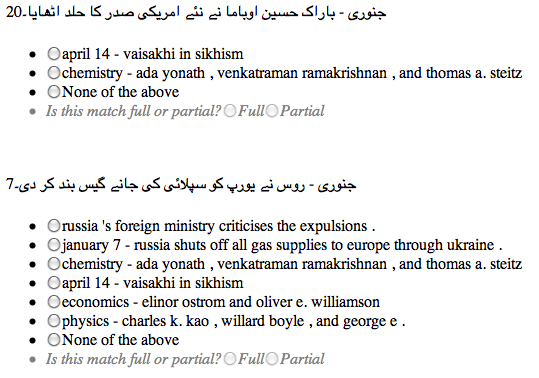
\includegraphics[scale=0.5]{images/turk_hit.png}
\caption{The MTurk annotation interface for finding Urdu-English parallel sentences.}
\label{fig:alignment_hit}
\end{center}
\end{figure}

Our method of pruning potential sentence pairs may leave us with more than ten
candidate English sentences for some Urdu sentences. When this happens, we make
additional questions about these Urdu sentences to ensure all candidate pairs
are accounted for in the annotation. 

In each HIT, we ask the Turkers to annotate up to ten Urdu sentences with their
English counterpart (if any), including two control questions with sentences
taken from the parallel data described in Section \ref{sec:turk_data}. There is
one positive and one negative control in each HIT. We also request that each HIT
be done by three Turkers.

\subsection{Data Collection Results}
\label{sec:turk_results}
In our first large-scale experiment, we took 92 Urdu-English article
pairs, applied our filters as described in Section \ref{sec:turk_data}, and
uploaded our task to MTurk. While there were over 8 million possible sentence
pairs in these articles before pruning, we ended up with $785,000$ sentence
pairs to be annotated at a total cost of $\$726.80$ (this cost includes the duplicate
annotations).

Agreement among the Turkers was high ($\kappa = 0.84$). While the most common
answer was ``None of the above'', there were a substantial number of Urdu
sentences which the Turkers found some English counterpart for. For $21.4\%$ of Urdu
sentences, at least one Turker found one of the English sentences to be
parallel, and in $44.8\%$ of Urdu sentences, at least two Turkers identified a match.

% thesis-only: Using this as a way to get parallel data

\subsection{Evaluation Using Partial Alignments}
\label{sec:partial}
When we evaluate our sentence pair alignment model, we would like to compute the
precision and recall of the proposed sentence alignments. However, since we
prune many possible sentence pairs before asking the Turkers for annotation, we
cannot be sure whether or not some sentence pairs are parallel. In this section,
we will outline a scheme for evaluating sentence alignments using our partially
annotated data.

Our primary intrinsic evalutaion metric is alignment F-measure on sentence
alignments. This metric could also be seen as F-measure on a parallel sentence
pair retrieval task. Let $T$ be the set of true positives (sentence pairs that
are truly parallel), and $P$ be the set of predicted positives (sentence pairs
identified by our model as parallel). Precision, recall, and F-measure are
defined as follows:

\begin{align*}
\mbox{Precison}&=& \frac{|T \cup P|}{|P|}\\
\mbox{Recall}&=& \frac{|T \cup P|}{|T|}\\
\mbox{F-measure}&=& \frac{2 \cdot \mbox{Precision} \cdot
\mbox{Recall}}{\mbox{Precision} + \mbox{Recall}}
\end{align*}

When our document pairs are only partially annotated, we will used modified
definitions of precision, recall, and F-measure. Let $U$ be the set of sentence
pairs which were not annotated as parallel or non-parallel.

\begin{align*}
\mbox{Precison}&=& \frac{|T \cup P|}{|P \setminus U|}\\
\mbox{Recall}&=& \frac{|T \cup P|}{|T|}\\
\mbox{F-measure}&=& \frac{2 \cdot \mbox{Precision} \cdot
\mbox{Recall}}{\mbox{Precision} + \mbox{Recall}}
\end{align*}

Since $T$ and $U$ are disjoint, only the definition of precision needs to
be modified. 

Given the annotations we gathered from MTurk, it is possible to define $U$ in
multiple ways. The most conservative method would be to take $U$ to be all
sentence pairs not presented to the Turkers. However, if we make the assumption
that sentence alignments of the document pairs are $1:1$, then when a Turker
annotates a sentence pair $(S, T)$ as parallel, it follows that all $(S, T')$
pairs with $T' \neq T$ and $(S', T)$ pairs with $S' \neq S$ are not parallel.
Since the alignments we found were mostly $1:1$, we decided to go with this
option.\footnote{There were a small number of alignments which were not $1:1$,
most of which were image captions.} Figure \ref{fig:partial_align} illustrates
this method.

\begin{figure}
\begin{center}
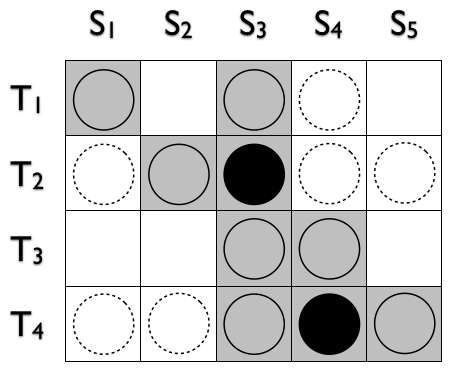
\includegraphics[scale=0.5]{images/partial_alignment.png}
\caption{A partial alignment grid for a comparable document pair. The shaded
cells in the grid represent the sentence pairs which were presented to the
Turkers for annotation. A filled circle indicates the Turker found the sentence
pair to be parallel, and an empty circle means the pair is not parallel. The
dashed circles represent the sentence pairs we infer to be non-parallel by
assuming the sentence alignments are $1:1$.}
\label{fig:partial_align}
\end{center}
\end{figure}

\subsection{Alternate Evaluation Strategies}
% thesis only
Section \ref{sec:partial} describes a method for using Turkers' partial
annotation of a document pair's sentence alignment for intrinsic evaluation of a
sentence alignment model. In this section, we will explore other
strategies for using the Turkers' output for evaluation.

In our MTurk task setup (see Section \ref{sec:design}), we collect redundant
annotations for each HIT. While this was done primarily for quality control, and
it is more convenient to use a single judgement for each sentence pair, we can
perform a more fine-grained analysis by looking at the individual Turkers'
judgements. Also, we gave the option of labeling a parallel sentence pair as a
``partial'' or ``full'' match.

\NoteJS{TODO: For the semi-supervised experiments, we want to treat sentence
pairs that any annotator marked as a match as a true positive. We could also
measure the inter-annotator agreement of our system against the Turkers.}

\section{Experiments}
\label{sec:unsup_experiments}
Our first set of experiments uses a semi-supervised setting. We have both
parallel sentences (labeled data) and comparable document pairs (unlabeled data),
and learn our model's parameters from both of these resources.

Our parallel corpus is taken from the NIST MT09 Urdu-English training set
and the bilingual dictionaries and sentences gathered by
\citet{Post12}.\footnote{This is the same parallel corpus used to create the
sentence pair filters used in collecting the annotated sentence alignments.}
The parallel sentences from this corpus are treated as single sentence document
pairs. Alternatively, the entire training set could be seen as a single document
pair whose sentence alignment lies completely on the diagonal. The model
described in \ref{sec:alignment} does not differentiate between these two ways
of viewing the corpus. In either case, learning from the parallel sentences is
identical to IBM Model 1 training.

The comparable document pairs are a subset of the Wikipedia article pairs that
we annotated using MTurk as described in Section \ref{sec:data}. $60\%$ of this
data was taken as a development set. The remaining $40\%$ of the annotated
document pairs was split into two equal sized test sets.\footnote{This split was
done in order to have training, development, and test sets for supervised
sentence aligment models.}

In the following experiments the setup is as follows: We initialize our
parameters by running five iterations of EM on the parallel sentences from our
labeled data. Then we run several iterations of EM on both the labeled data and
unlabeled data, measuring performance after each iteration.

\subsection{Intrinsic Results}

\subsection{Extrinsic Results}
\NoteJS{This experiments section takes the new strategy where we start with lots
of supervision and then see how well we do as we remove data. Hopefully it will
end with good unsupervised results.}
The ultimate goal of parallel sentence extraction is to improve the quality of
end-to-end machine translation. In this section we will measure MT performance
before and after the extracted parallel sentences are added to the training
data.

\subsubsection{Corpora}
\begin{table*}
\small
\begin{center}
\begin{tabular}{|c|c|c|c|c|c|c|c|}
\hline
French & German & Polish & Italian & Dutch & Portuguese & Spanish & Japanese \\
496K & 488K & 384K & 380K & 357K & 323K & 311K & 252K\\
\hline
Russian & Swedish & Finnish & Chinese & Norwegian & Volap\"{u}k & Catalan & Czech \\
232K & 197K & 146K & 142K & 141K & 106K & 103K & 87K\\
\hline
\end{tabular}
\end{center}
\caption{The sizes of corpora in tokens and sentences for the Spanish-English
condition.}
\label{table:esen_corpora}
\end{table*}

\section{Experiments (Alternate)}
\label{sec:experiments_all}
In this section, we explore the relationship between the amount of initial
parallel data, the quality of the extracted parallel data, and the end-to-end
machine translation quality. We start with Spanish-English as our language pair,
since this is a high resource language pair, and we can always simulate a low
resource setting by restricting the amount of data used.

\subsection{Datasets}
For our initial parallel data, we use the parallel and monolingual corpora
available for the 2010 Machine Translation Workshop's shared task (WMT10). For
the Spanish-English task, the WMT10 data includes Europarl version 5 (we use
version 6 in our experiments\NoteJS{This may change to 7}) \citep{Koehn05}, the United Nations
parallel text, and parallel and monolingual news corpora. Table \ref{table:esen_parallel}
lists the corpora used in detail.

\begin{table*}[ht]
\begin{center}
\begin{tabular}{|rr||r|r|r|}
\hline
      &                & Spanish        & English & English (Monolingual) \\
\hline
\textbf{Europarl} \
      & Sentences     & 1.79M       & 1.79M   & 1.79M   \\
      & Tokens     & 46.8M       & 44.7M   & 44.7M   \\
\hline
\textbf{United Nations} \
      & Sentences     & 6.22M       & 6.22M & 6.22M     \\
      & Tokens     & 191M       & 164M & 164M     \\
\hline
\textbf{News Commentary} \
      & Sentences     & 98.6K       & 98.6K & 126K      \\
      & Tokens     & 2.45M       & 2.10M  & 261M    \\
\hline
\textbf{News} \
      & Sentences     & N/A       & N/A & 48.7M     \\
      & Tokens     & N/A       & N/A & 989M     \\
\hline
\end{tabular}
\end{center}
\caption{Statistics for the initial parallel/monolingual data used in training
baseline MT systems and for extracting new parallel data. The monolingual data
is only used for language modeling, not for extracting parallel sentences.}
\label{table:esen_parallel}
\end{table*}

This data is used both for training the parallel sentence extractor, and as the
initial data in the MT system.

\subsection{Supervised Parallel Sentence Extraction}
In order to extract parallel sentence pairs from Wikipedia, we used a simplified
version of the approach described in \citet{Smith10}.

Using the initial parallel data and a small amount of annotated Spanish-English
Wikipedia articles, we extracted sentence pairs from all of the Spanish-English
Wikipedia articles which were identified as sharing a topic through Wikipedia's
Interwiki link system. This gave us a set of 433 thousand comparable document
pairs. For all pairs of sentences in each document pair, we applied a binary
classifier to determine whether or not the sentence pair was parallel.

Table \ref{table:esen_wiki_parallel} lists the parallel corpora extracted from
Spanish-English article pairs from Wikipedia. ``Wiki@X'' refers to the parallel
sentences extracted with a classification threshold of $X$ (a lower
classification threshold will allow more sentences to be extracted). The
monolingual data was taken from the English side of all Spanish-English document
pairs, making it consistent across conditions.

\begin{table*}[ht]
\begin{center}
\begin{tabular}{|rr||r|r|r|}
\hline
      &                & Spanish        & English & English (Monolingual) \\
\hline
\textbf{Wiki@0.75} \
      & Sentences     &   ---     & --- & 14.8M     \\
      & Tokens     &  ---      & --- & 286M    \\
\hline
\textbf{Wiki@0.5} \
      & Sentences     & 1.60M       & 1.60M & 14.8M     \\
      & Tokens     & 44.8M       & 51.0M & 286M     \\
\hline
\textbf{Wiki@0.25} \
      & Sentences     &   ---     & --- & 14.8M     \\
      & Tokens     &  ---      & --- & 286M    \\
\hline
\end{tabular}
\end{center}
\caption{Statistics for parallel corpora extracted from Wikipedia.}
\label{table:esen_wiki_parallel}
\end{table*}

\subsection{Results}
We report end-to-end MT results using the initial parallel data and the
extracted parallel data from Wikipedia. For our baseline MT system we used the
phrase-based model included in the Moses toolkit \citet{Koehn07} with all
options set to the default. % TODO: Cite Edinburgh submission

We used two test sets to evaluate the end-to-end MT performance: the test set
from WMT10 which was taken from the news domain, and a set of parallel sentences
from Wikipedia gathered by \citep{Smith10}.

\begin{table*}[ht]
\begin{center}
\begin{tabular}{|r||r|r|}
\hline
      & WMT10        & Wikipedia \\
\hline
\textbf{Europarl Only} \
      & 24.75       & ---    \\
\textbf{+Wiki LM} \
      & 26.91       & ---    \\
\textbf{+Wiki Parallel (@0.75)} \
      & ---       & ---    \\
\textbf{+Wiki Parallel (@0.5)} \
      & 27.41       & ---    \\
\textbf{+Wiki Parallel (@0.25)} \
      & ---       & ---    \\
\hline
\textbf{All Initial Corpora} \
      & 28.51       & ---    \\
\textbf{+Wiki LM} \
      & 28.55       & ---    \\
\textbf{+Wiki Parallel (@0.75)} \
      & ---       & ---    \\
\textbf{+Wiki Parallel (@0.5)} \
      & 29.23       & ---    \\
\textbf{+Wiki Parallel (@0.25)} \
      & ---       & ---    \\
\hline
\end{tabular}
\end{center}
\caption{BLEU scores for systems trained on different sets of parallel and
monolingual data before and after adding data from Wikipedia.}
\label{table:esen_bleu}
\end{table*}

\section{Conclusions}



%\setcounter{chapter}{5}
%\chapter{Mining Parallel Data from the Web}
\label{chap:web}



% TODO: Remove this in the final version
%\setcounter{chapter}{6}
%\chapter{Scraps}
Text that will be cleaned up and integrated somewhere.

\section{HTML Data Cleaning}
In this work we are interested in finding parallel sentences in multilingual
websites. A non-trivial step in this process is identifying sections of a website
which contain useful text, while removing ``boilerplate'' information such as
menus. This task, which is common part in many systems which use the web as a
corpus, has been explored in the CleanEval competition \citep{CleanEval}. This
section will explore the different approaches used for boilerplate
identification in CleanEval and other work.

\subsection{CleanEval}
CleanEval \citep{CleanEval} is a shared task on cleaning web pages. 

% ------------------------------------------------------------------------------
\section{Web Mining Pipeline}

\paragraph{Language Identification}
The documents from the previous step are annotated with their language, which
was identified based only on the URL. Since searching for language codes in a
URL cause many false positives (the two letter language code for Indonesian is
``id''), we apply a language identification system to the text of the document
to ensure that the URL matching was correct. 

The method we use for language identification is Prediction by Partial Matching
(PPM) \citep{Cleary84}.\footnote{Thanks to Paul McNamee
({\tt paul.mcnamee@jhuapl.edu}) for providing the code and data.} For each
language, we train a character $n$-gram model on text. At test time, we apply
the $n$-gram model for each language to the text of a document. The model which
assigns the highest score to the text is taken as the correct language.

\NoteJS{Paul's data came from a source that can't be redistributed. I could
re-train models on Wikipedia to make the whole pipeline more reproducible, and
this would let me have a small results section here.}
\NoteJS{Given Wikipedia, we could train binary classifiers for each language,
and that may be more effective. I'll come back to this if language ID becomes a
problem.}

\paragraph{Sentence Filtering}
Since we do not perform any boilerplate removal in earlier steps, there are many
sentence pairs produced by the pipeline which contain menu items or other bits
of text which are not useful to an MT system. To remove this data, we prune
segment pairs unless both segments contain at least 5 tokens composed of
alphanumeric characters only, and end with punctuation.


% TODO: Switch back to IEEE for final submission
%\bibliographystyle{IEEEtran}
\bibliographystyle{plainnat}
\bibliography{refs}

\end{document}
